\part{Misura della lunghezza d'onda di un laser He-Ne } \label{part:Ottica_1A}

\section{Strumentazione}
La strumentazione impiegata per questa misura prevede l'uso di:
\begin{list}{}
\item \textbf{un calibro ventesimale}, del quale abbiamo impiegato la sola scala graduata del righello come reticolo
di diffrazione  (passo reticolare $d = 1 \; mm$);
\item \textbf{un laser He-Ne} : sorgente del quale vogliamo misurare la frequenza;
\item \textbf{uno specchio} col quale orientare il fascio emesso dal laser.
\item \textbf{uno schermo} dove osservare e misurare le frange di diffrazione prodotte dal reticolo;
\item \textbf{un metro a nastro} (risoluzione $1 \; mm$) col quale misurare la distanza tra il reticolo di 
diffrazione e lo schermo;
\item \textbf{un righello} (risoluzione $1 \; mm$) per misurare le distanze tra le frange sullo schermo.
\end{list}
\bigskip


\begin{figure} [!h]
	\centering
	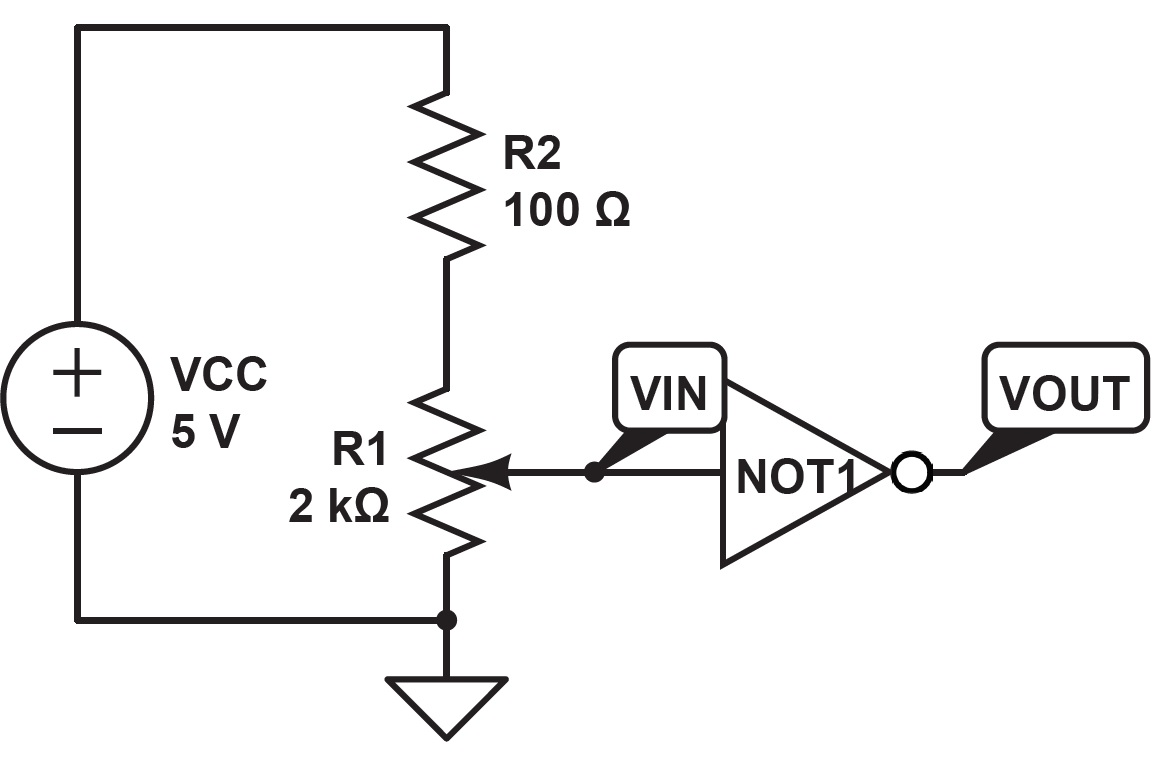
\includegraphics[width=0.9\textwidth]{./pictures/immagine1}
	\caption{Schema dell'apparato impiegato per la misura $\Lambda$.}
	\label{fig:schema_appar}
\end{figure}
In \figurename{ \ref{fig:schema_appar}} è riportato lo schema dell'apparato sperimentale impiegato. 